\documentclass[sigconf,screen]{acmart}

\usepackage{caption}
\usepackage{subcaption}

%%
%% \BibTeX command to typeset BibTeX logo in the docs
\AtBeginDocument{%
  \providecommand\BibTeX{{%
    \normalfont B\kern-0.5em{\scshape i\kern-0.25em b}\kern-0.8em\TeX}}}

%% Rights management information.  This information is sent to you
%% when you complete the rights form.  These commands have SAMPLE
%% values in them; it is your responsibility as an author to replace
%% the commands and values with those provided to you when you
%% complete the rights form.
%%% The following is specific to ESEC/FSE '19-SRC and the paper
%%% 'Understanding Source Code Comments at Large-Scale'
%%% by Hao He.
%%%
\setcopyright{rightsretained}
\acmPrice{}
\acmDOI{10.1145/3338906.3342494}
\acmYear{2019}
\copyrightyear{2019}
\acmISBN{978-1-4503-5572-8/19/08}
\acmConference[ESEC/FSE '19]{Proceedings of the 27th ACM Joint European Software Engineering Conference and Symposium on the Foundations of Software Engineering}{August 26--30, 2019}{Tallinn, Estonia}
\acmBooktitle{Proceedings of the 27th ACM Joint European Software Engineering Conference and Symposium on the Foundations of Software Engineering (ESEC/FSE '19), August 26--30, 2019, Tallinn, Estonia}

\begin{document}

%%
%% The "title" command has an optional parameter,
%% allowing the author to define a "short title" to be used in page headers.
%\title{Source Code Comments in Open Source Projects}
\title{Understanding Source Code Comments at Large-Scale}

%%
%% The "author" command and its associated commands are used to define
%% the authors and their affiliations.
%% Of note is the shared affiliation of the first two authors, and the
%% "authornote" and "authornotemark" commands
%% used to denote shared contribution to the research.

\author{Hao He}
\affiliation{%
  \institution{Peking University, China}
  \country{}}
\email{heh@pku.edu.cn}

\begin{abstract}
Source code comments are important for any software, but the basic patterns of writing comments across domains and programming languages remain unclear. In this paper, we take a first step toward understanding differences in commenting practices by analyzing the comment density of 150 projects in 5 different programming languages. We have found that there are noticeable differences in comment density, which may be related to the programming language used in the project and the purpose of the project.
\end{abstract}

\begin{CCSXML}
<ccs2012>
<concept>
<concept_id>10011007.10011074</concept_id>
<concept_desc>Software and its engineering~Software creation and management</concept_desc>
<concept_significance>500</concept_significance>
</concept>
</ccs2012>
\end{CCSXML}

\ccsdesc[500]{Software and its engineering~Software creation and management}

\keywords{Source Code Comments, Comment Density, Empirical Study}

%%
%% By default, the full list of authors will be used in the page
%% headers. Often, this list is too long, and will overlap
%% other information printed in the page headers. This command allows
%% the author to define a more concise list
%% of authors' names for this purpose.

%%
%% This command processes the author and affiliation and title
%% information and builds the first part of the formatted document.
\maketitle

\section{Problem and Motivation}

%Source code comments constitute an important part of any software, which help people understand the code and facilitate the maintenance.
%To understand how programmers write comments and find insights for improving software quality, existing studies have analyzed comments in open source projects from different perspectives, such as software reliability\cite{2009ICSE-Listening}, comment code co-evolution\cite{Fluri2009Coevolution}, and the purpose of comments\cite{2017MSR-ClassifyingJavaComment}. However, these studies are often limited in one programming language, one or several projects and only focus on one special aspect of code comments. Recently, the rise of large open source platforms such as GitHub and the emergence of open source project databases like GHTorrent\cite{2012MSR-GHTorrent} and World of Code\cite{2019MSR-WorldOfCode} enables large scale analysis of open source projects. On the other hand, recent advancement in mining code comment pairs and automatic code generation are often based on a large dataset of open source projects and requires deep understanding of comments in these projects. Therefore, a large scale investigation of comments in open source projects is desired.

Source code comments constitute an important part of any software, which help people understand code and facilitate software maintenance~\cite{Woodfield:1981:EMC:800078.802534,Tenny:1988:PRP:51199.51203}.
To understand how programmers write comments and find insights for improving software practices, existing studies have analyzed comments from various perspectives, such as %software reliability~\cite{2009ICSE-Listening} (how this is related to comments?), 
ratio of comments~\cite{POman1992ICSM}, comment code co-evolution~\cite{Fluri2009Coevolution}, and the purpose of comments~\cite{2017MSR-ClassifyingJavaComment}. 
However, these studies are often limited in one programming language, one or several projects and one specific aspect of code comments.  
Meanwhile, the very basic pattern of writing comments across domain and language remains unclear, while it may greatly help software projects understand their position and adjust their practices accordingly.
The main reason might be that it is not easy to access sufficient projects to make a comparison. In particular, we may not be able to access a large amount of projects and the effort to collect the needed data is significant.
Recently, the rise of large open source platforms such as GitHub and the emergence of open source project databases like GHTorrent~\cite{2012MSR-GHTorrent} and World of Code~\cite{2019MSR-WorldOfCode} enable large scale analysis of software projects. %On the other hand, recent advancement in mining code comment pairs and automatic code generation are often based on a large dataset of open source projects and requires deep understanding of comments in these projects. Therefore, a large scale investigation of comments in open source projects is desired.
Therefore, we set up to conduct a large scale investigation of code comments and expect to help practices in various ways, e.g., defining benchmark for comment density, locating where to comment, and generating comments for code.
%In this research abstract, we take an initial step toward understanding differences in comment usage patterns in open source projects by addressing the following research questions
%\begin{itemize}
%\item RQ1: Is there any difference in comment usage patterns in different projects?
%\item RQ2: If there are any differences, what are the differences and what caused the differences?
%\end{itemize}

% \vspace{-0.3cm}
\section{Background and Related Work}
Programmers frequently write comments along with source code. As a result, code comments form an important part of documentation, providing additional information not immediately visible from source code. Studies have shown that reading source code with comments aid with program comprehension~\cite{Woodfield:1981:EMC:800078.802534,Tenny:1988:PRP:51199.51203}. 
%The ratio of comments has also been proposed as one of the metrics for software maintainability~\cite{POman1992ICSM} and code quality~\cite{StamelosAOB02CodeQualityAnalysis}. 
Further research reveals that the quality of comment itself, especially the consistency between source code and comments, is crucial for avoiding software bugs and improving maintainability~\cite{Fluri2009Coevolution, Tan:2007:IBB:1294261.1294276}.

Because of the important role of comments in program comprehension, software quality and software maintenance, there have been a number of studies that analyze comments in existing software projects~\cite{2009ICSE-Listening,2009ICSECommentDensity,Fluri2009Coevolution,2011ESEM-CommentsInJava,2017MSR-ClassifyingJavaComment,2019Arxiv-LinksInComments}. However, existing studies either focus on one programming language~\cite{2011ESEM-CommentsInJava,2017MSR-ClassifyingJavaComment} or  one specific application domain(e.g. operating systems~\cite{2009ICSE-Listening}), or consider only one specific dimension of comments (e.g. comment density~\cite{2009ICSECommentDensity}, links in comments~\cite{2019Arxiv-LinksInComments}). To the best of our knowledge, no existing research has focused on analyzing commenting practices and their differences in a large number of heterogeneous projects.

%Recently, considerable efforts have been taken in developing methods for mining code comment pairs and automatic comment generation (e.g. \cite{2016ACL-SummarySourceCode,2018ICPC-DeepCodeComment,2018ICJAI-SummarizeSourceCodeWithAPIKnowledge,2013ASE-MiningQASites,2018ASE-NeuralFrame}). For example, \cite{2018ICPC-DeepCodeComment} employs a deep learning based comment generation framework and uses 9714 Java projects from GitHub as its dataset.  GHTorrent~\cite{2012MSR-GHTorrent} and World of Code~\cite{2019MSR-WorldOfCode} are two examples of open source project database for research purposes.

% \vspace{-0.3cm}
\section{Approach}
We take an initial step towards understanding commenting practices across projects by addressing the following research questions:
\begin{itemize}
\item RQ1: Do projects practice commenting differently?
\item RQ2: What may cause the differences?
\end{itemize}

\subsection{Selection of Open Source Projects}
We choose five most popular programming languages among 1000 most starred Repositories on GitHub (JavaScript, Java, C++, Python and Go at the time of April 2019) and collect 30 most starred repositories for each programming language. This is a relatively small dataset for preliminary analysis and we plan to use the World of Code~\cite{2019MSR-WorldOfCode} database in the future.

\subsection{Analysis of Comment Density}
To answer RQ1, we begin from one simple metric: comment density, which has also been used to measure software maintainability~\cite{POman1992ICSM} and quality~\cite{StamelosAOB02CodeQualityAnalysis}.
We plan to investigate more sophisticated metrics in the future, such as vocabulary used in comments and distribution of comments over program structures. %The investigation of comment density is inspired by~\cite{2009ICSECommentDensity}, which attempts to find correlations between comment density and other factors. However, it considers all the projects as the same and does not consider the inherent differences among projects. %

We define comment density of a project as follows:
\begin{equation}
    \mbox{Comment Density} = \frac{\mbox{Line of Comments}}{\mbox{Line of Code}}
\end{equation}
For each project, we count its lines of code and lines of comment of its major programming language. 
%We have found that comment density indeed vary greatly in the 150 collected projects($avg=0.2124, stddev=0.1807, max=1.2691, min=0$). Therefore, further investigation is needed to find out what factors might contribute to the difference.

To answer RQ2, we propose the following hypothesis based on existing literature and practical experiences:
\begin{enumerate}
    \item H1: The programming language used in a project may affect its comment density.
    \item H2: The purpose (domain) of a project may affect its comment density.
    \item H3: Team size may affect the comment density of a project because more people need to read the code.
\end{enumerate}

\begin{figure}
    \begin{subfigure}[b]{0.2\textwidth}
        \centering
        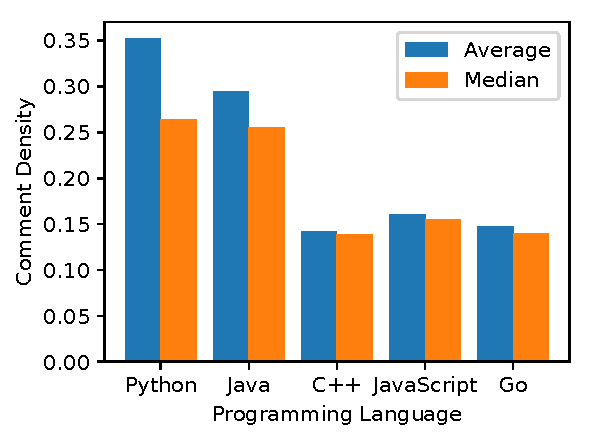
\includegraphics[width=\textwidth]{figs/cd_by_lang.pdf}
        \caption{Comment density in different programming languages}
        \label{fig:cd_lang}
    \end{subfigure}
    \begin{subfigure}[b]{0.2\textwidth}
        \centering
        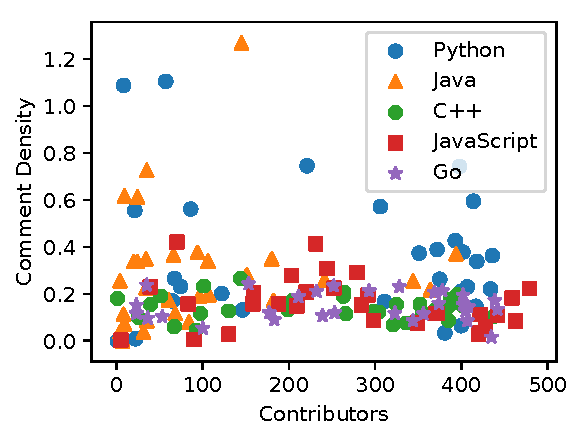
\includegraphics[width=\textwidth]{figs/cd_contrb.pdf}
        \caption{Relationship between comment density and \# of contributors}
        \label{fig:cd_contrib}
    \end{subfigure}
    \caption{Figures for Comment Density Analysis}
\end{figure}

%\section{Results and Contributions}
\section{Results}

%\subsection{Addressing Our Research Questions}
%\textbf{RQ1: Is there any difference in comment usage patterns in different projects?} 
\textbf{RQ1: Do projects practice commenting differently?}
We find that comment density varies greatly in the 150 collected projects ($avg=0.2124, stddev=0.1807, max=1.2691, min=0.003$, excluding projects with no code at all). The most heavily commented project has more lines of comments than source code (which is java-design-patterns\footnote{\url{https://github.com/iluwatar/java-design-patterns}}, with 29414 lines of code and 37329 lines of comments). On the other hand, comments in some projects are extremely scarce, e.g., Font-Awesome\footnote{\url{https://github.com/FortAwesome/Font-Awesome/}}, with 73808 lines of code and 240 lines of comments. The results suggest that projects do have different commenting practices. %Therefore, further investigation is needed to find out what factors might contribute to the difference.
%It indicates that there are indeed differences in comment usage patterns in different projects. 
%Further investigation is needed on the difference of comment usage patterns in different open source projects.
%可以解释一下这个结果. 例如,0和1.2691到底有多大差距, 是否suggest anything

%\textbf{RQ2: If there are any differences, what are the differences and what caused the differences?} 
\textbf{RQ2: What may cause the differences?}
%From our preliminary analysis on comment density, we have found that comment density vary greatly across different projects. Also, we've found that the programming language used in one project will affect its comment density. Whether the project is set up for educational purpose, software reuse or direct application probably have an effect on its comment density. The relationship between comment density and project size/contributor size needs further investigation.

To confirm H1, we plot the average and median comment density for different programming languages (Figure~\ref{fig:cd_lang}). Since the distribution is not normal, we conduct Wilcoxon signed-rank test on languages pairs and find that the comment density of Python and Java projects is significantly higher than C++, JavaScript and Go projects(See Table \ref{tab:pvalue} for original p-values). One possible explanation is that there are widely adopted documentation generation tools for Java~\cite{Javadoc} and Python~\cite{Sphinx}, which specify a given set of rules for programmers to write comments. The other three languages, however, have no widely adopted rules for writing comments.

\begin{table}
  \caption{Original p-Values of the Wilcoxon Signed-rank Test}
  \label{tab:pvalue}
  \begin{tabular}{cccccc}
    \toprule
    &Python&Java&C++&JavaScript&Go\\
    \midrule
    Python&1.0000&0.4420&0.0003&0.0034&0.0008\\
    Java&&1.0000&0.0027&0.0115&0.0043\\
    C++&&&1.0000&0.7227&0.7562\\
    JavaScript &&&&1.0000&0.9764\\
    Go &&&&&1.0000\\
  \bottomrule
\end{tabular}
\end{table}

To confirm H2, we manually inspect 30 Java projects and 30 JavaScript projects in the collected dataset. We identify three major purposes for which the project is used:
\begin{enumerate}
    \item \textbf{Software Reuse}. The project is a framework or a library, which provides functions or solutions for other people to reuse in their own applications (e.g. Vue.js\footnote{\url{https://github.com/vuejs/vue}}, a progressive web framework for developers to build web applications).
    \item \textbf{Application}. The project is a complete and ready-to-use application for interested users (e.g. proxyee-down\footnote{\url{https://github.com/proxyee-down-org/proxyee-down}}, an HTTP downloader implemented in Java).
    \item \textbf{Education}. The project is set up for educational purposes. Users of this project are supposed to understand and learn from the source code (e.g. Android-CleanArchitecture\footnote{\url{https://github.com/android10/Android-CleanArchitecture}}, an example to learn how to architect an Android application).
\end{enumerate}

\begin{table}
  \caption{Average Comment Density by Project Purpose}
  \label{tab:cd_type}
  \begin{tabular}{cccc}
    \toprule
    &Education&Software Reuse&Application\\
    \midrule
    Java&0.5751&0.2739&0.0641\\
    JavaScript&0.2650&0.1760&0.1050\\
  \bottomrule
\end{tabular}
\end{table}

Table~\ref{tab:cd_type} summarizes average comment density of the three different type of projects, for Java and JavaScript respectively. Projects with educational purposes have the highest comment density, while projects which are ready-to-use applications have the lowest, and projects with software reuse purposes stay in the middle. One possible explanation is that, for educational projects, it is important to have enough comments so that most users can understand the code. For applications, only core developers need to read and understand its source code and only a minimum amount of comments are necessary. For reusable open source libraries and frameworks, users occasionally need to read its source code to understand its usage or find bugs, and thus they need to have a reasonable amount of comments. However, we have to point out that the dataset is too small to conduct any statistic significance tests. We plan to replicate on a larger dataset in the future.

To confirm H3, we plot the number of contributors along with comment density (Figure~\ref{fig:cd_contrib}). However, we fail to observe any correlation that supports H3. Further investigation is needed to reveal the relationship between comment density and team size. 

\section{Conclusion}
 
We take a first step toward understanding the differences of source code comments across various projects. 
We have found that there are indeed noticeable differences in comment density of different projects, which may be related to the programming language used in the project and the purpose of the project. The result is promising and we plan to further investigate this problem in the future. %if there is space, need to come back to the beginning picture: help practices in various ways, e.g., defining benchmark for comment density, locating where to comment, and generating comments for code.

%%
%% The next two lines define the bibliography style to be used, and
%% the bibliography file.
\bibliographystyle{ACM-Reference-Format}
\bibliography{references}

\end{document}
\endinput

